\newpage
\section{Proponowane rozwiązanie}
\subsection{Architektura systemu}

\subsection{Klasyfikacja}\label{klasyfikacja}
W celu dokonania klasyfikacji, z każdego nagrania wybrane zostają 3 sekwencje, składające się z 64 kolejnych klatek.
Rozkład wybranych sekwencji dokonany jest w taki sposób, aby były one rozłożone możliwie równomiernie. W przypadku gdy
długość
3 sekwencji przekracza długość nagrania, sekwencje mają części wspólne, w przeciwnym przypadku będą rozłączne.
Przykładowy podział na sekwencje został przedstawiony na rysunku \ref{fig:sekwencje}. Zaprezentowane w pracy modele
dokonują klasyfikacji sekwencji. Klasy nagrań zostają wybrane poprzez zsumowanie przewidzianych przez model
prawdopodobieństw dla każdej z sekwencji oraz wybranie klasy o największym prawdopodobieństw.
\begin{figure}[!h]
    \centering 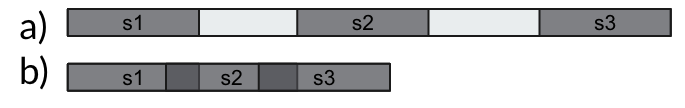
\includegraphics[width=0.75\linewidth]{sekwencje.png}
    \caption{Rozkład wybieranych sekwencji, a) łączna długość sekwencji mniejsza niż długość nagrania, b) łączna długość wybranych sekwencji przekracza długość nagrania - sekwencje mają części wspólne}
    \label{fig:sekwencje}
\end{figure}
\subsection{Wykorzystane cechy}
W pracy wykorzystane zostały trzy rodzaje cech wyekstrahowanych z klatek nagrania. Wykorzystane cechy zostały zwizualizowane na rysunku \ref{fig:wiz-cech}

Modele hierarchiczne biorące pod
uwagę aktywności wyselekcjonowanych osób wymagają dodatkowego przetworzenia wideo składającego się z następujących
kroków: \begin{itemize}
\item Detekcja osób w nagraniu
\item Śledzenie wykrytych osób
\end{itemize}
\begin{figure}[!h]
    \centering 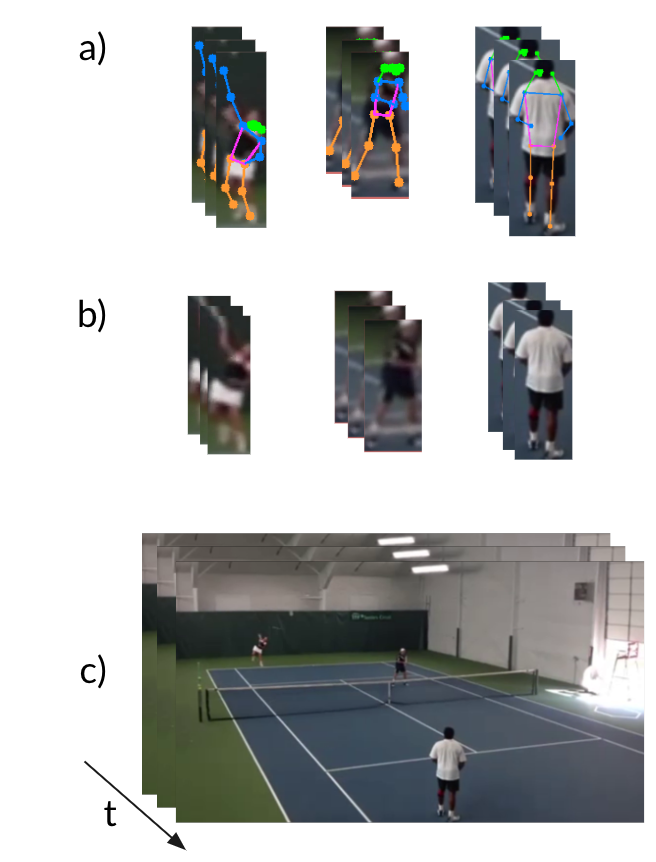
\includegraphics[width=0.70\linewidth]{features-vis.png}
    \caption{Wizualizacja cech użytych do reprezentacji sekwencji. a) cechy szkieletowe, b) cechy RGB pojedynczych osób, c) cechy RGB całego obrazu}
    \label{fig:wiz-cech}
\end{figure}
\subsubsection{Cechy szkieletowe}
Cechy szkieletowe wyekstrahowane zostały przy pomocy modelu YOLOv7-pose \cite{yolov7-pose}, z wycinków klatek
zawierających pojedyncze osoby. Sekwencja składająca się z cech szkieletowych reprezentowana jest przez wektor o
wymiarach $(N, T, 17, 2)$, gdzie pierwszy wymiar $N$ oznacza ilość osób na wejściu do modelu, $T$ liczbę badanych klatek,
natomiast 2 ostatnie wymiary oznaczają 17 dwuwymiarowych punktów reprezentujących szkielet.
\subsubsection{Cechy RGB pojedynczych osób}
Cechy RGB pojedynczych osób, wyekstrahowane zostały przy pomocy modelu mobilenet\cite{mobilenet}, zakończonego warstwą
AveragePooling'u z wycinków klatek zawierających pojedyncze osoby. Sekwencja składająca się z cech RGB pojedynczych
osób, reprezentowana jest przez wektor o wymiarach $(N, T, 256)$, gdzie $N$ oznacza ilość osób na wejściu do modelu, $T$ liczbę badanych klatek, 256 to rozmiar wektora zakodowanych cech RGB wyznaczonych przez model mobilenet zredukowany przy
pomocy algorytmu analizy głównych składowych PCA z oryginalnego wymiaru wynoszącego 960.  
\subsubsection{Cechy RGB całego obrazu}\label{sekwncje-klatek}
Cechy RGB całego obrazu, wyznaczone zostały przy pomocy tej samej metody co w przypadku pojedynczych osób, różnią
się tylko tym, że badany jest cały obraz zamiast pojedynczej osoby. Tego typu sekwencja reprezentowana jest przez wektor
o wymiarach $(T, 256)$, gdzie $T$ oznacza liczbę badanych klatek, 256 to rozmiar wektora RGB ~
\subsection{Hiper-parametry sekwencji}
\subsubsection{Liczba osób na wejściu do modelu}\label{kryteria-wyboru}
Liczba osób na wejściu do modelu,
reprezentowana w ww. wektorach przez literę $N$, w przeprowadzonych eksperymentach wynosi 6. Wartość ta wyznaczona została
poprzez wyliczenie średniej ilości wykrytych osób we wszystkich przetworzonych klatkach w całym zbiorze danych. Parametr ten ma również duże znaczenie na rozmiar danych treningowych modelu. 

Aby osoba mogła zostać zaliczona do sekwencji, musi znajdować się w co najmniej 70\% klatek sekwencji. Warunek ten 
wynika z możliwości wystąpienia następujących sytuacji: \begin{itemize} 
\item Osoba może pojawić się w polu widzenia kamery dopiero pod koniec sekwencji np. wbiec
\item Detektor może zgubić ślad osoby
\item Poruszająca się kamera, śledząca akcje może uchwycić chwilowo osobę stojącą w tle 
\end{itemize} 
W powyższych przypadkach istnieje duże prawdopodobieństwo, że taka osoba nie wnosi informacji o dziejącej się akcji i może stanowić 
tylko szum na wejściu modelu. W przypadku, gdy wykryta osoba spełnia ten warunek, ale nie występuje na wszystkich 
klatkach badanej sekwencji, jej brakujące klatki zostają uzupełnione poprzez powielenie najbliższej dostępnej klatki. 

W ten sposób przetworzony 
zbiór wykrytych osób zostaje posortowany w ramach ich sekwencji według ich największego otaczającego prostokąta, oraz 
z pierwszych $N$ osób zostaje zbudowany wektor wejściowy. Tego typu sortowanie ma na celu wybranie osób na pierwszym  
planie, który najprawdopodobniej niesie najwięcej informacji o odbywającej się akcji. 

W przypadku, gdy w sekwencji bierze udział mniej niż N osób, brakująca część wektora zostaje uzupełniona zerami. Badane
są tylko sekwencje, w których występuje co najmniej jedna osoba. 

\subsubsection{Długość sekwencji}
Długość sekwencji $T$ oznacza liczbę klatek przedstawiających akcje, z których zostały wyekstrahowane cechy. W pracy przyjęta została wartość 64, jako że wszystkie nagrania w badanym zbiorze danych składają się z częstotliwości 30 klatek na sekundę badane są sekwencje około 2 sekundowe. Sekwencje budowane są z następujących po sobie klatkach. 

\subsection{Architektura systemu}
Architektura systemu klasyfikującego, razem ze wstępnym przetworzeniem danych oraz wykorzystanymi modelami została przedstawiona na rysunku \ref{fig:architektura}.

Na wejściu system przyjmuje surowe, nieprzetworzone w żaden sposób nagranie, które podawane jest procesowi ekstrakcji cech. Etap ten na rysunku \ref{fig:architektura} został zaznaczony liniami przerywanymi, ze względu na to, że jest on wymagany tylko w przypadku, gdy model klasyfikujący bierze pod uwagę akcje pojedynczych osób (modele hierarchiczne), dla modelu badającego cechy całego obrazu krok ten może zostać pominięty. Dysponując tak przetworzonymi danymi, wybierane są sekwencje nagrania, które są wejściami do klasyfikatora.
\begin{figure}[!h]
    \centering 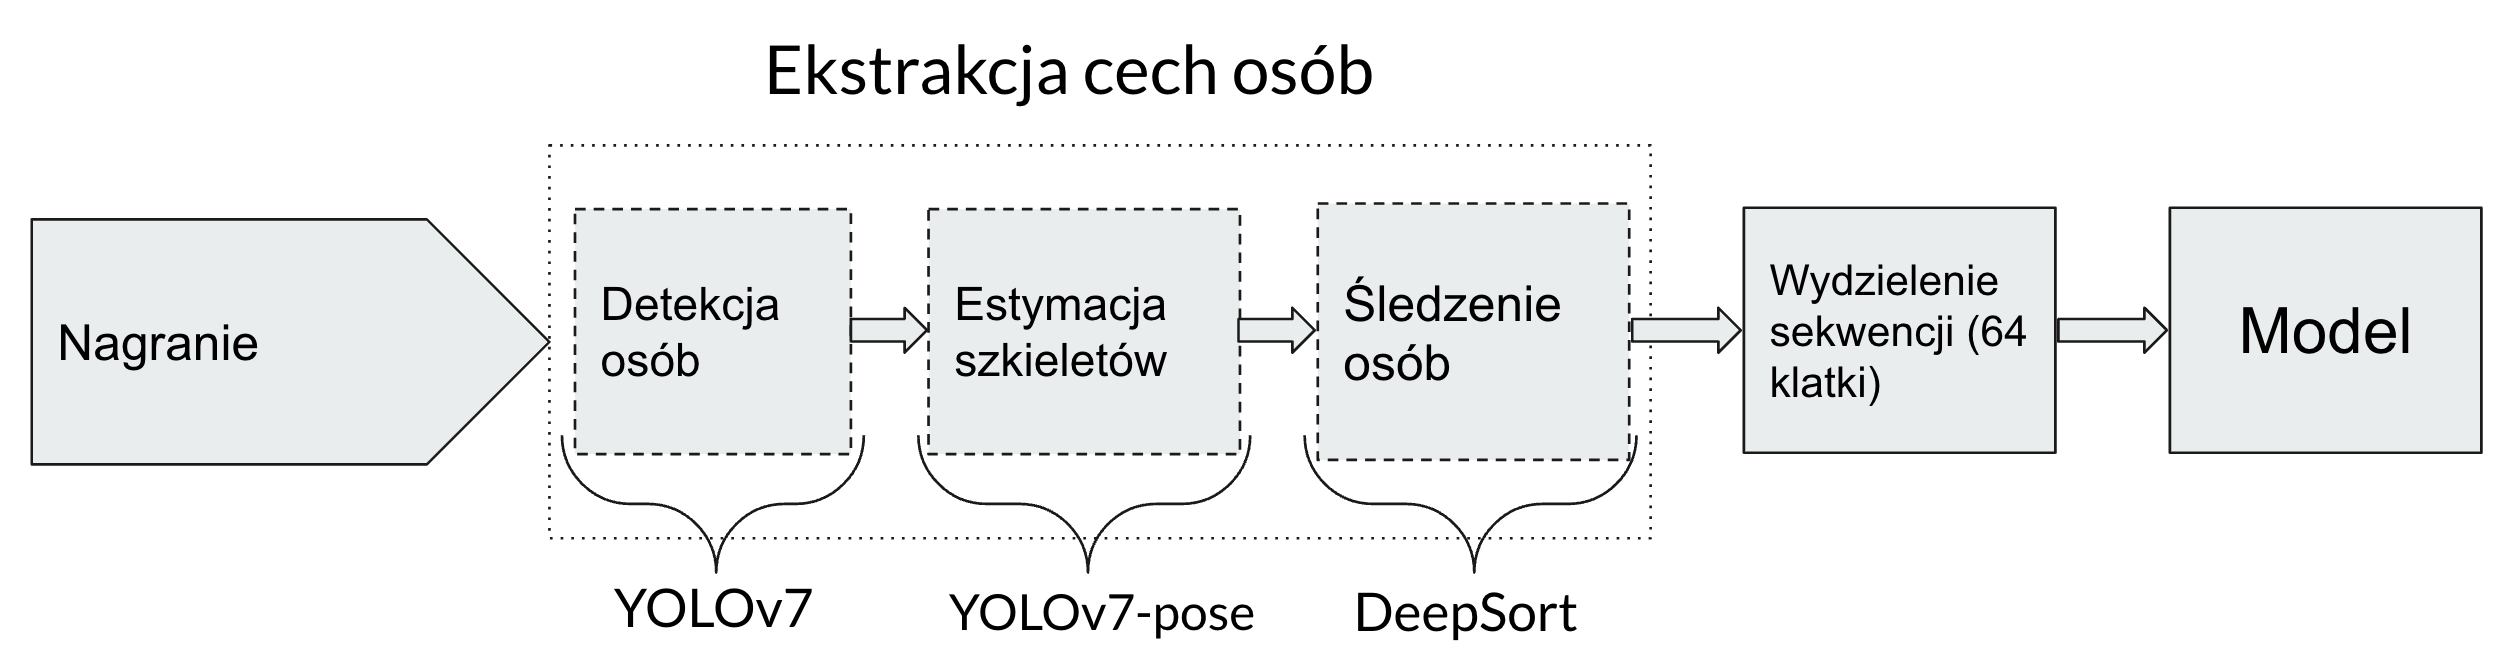
\includegraphics[width=0.90\linewidth]{architektura.png}
    \caption{Graf przedstawiający architekturę systemu}
    \label{fig:architektura}
\end{figure}
\subsubsection{Detekcja osób oraz estymacja szkieletów}
Detekcja osób w nagraniu odbywa się przy pomocy modelu YOLOv7 \cite{yolov7}. Jest to najlepszy dostępny detektor,
dostępny na moment implementacji systemu. Jego główna zaleta polega na tym, że wykonuje cały proces detekcji jednocześnie, bez potrzeby wielokrotnego analizowania obrazu, co sprawia, że jest bardzo szybki. YOLO dzieli obraz na siatkę komórek i dla każdej komórki przewiduje obiekt znajdujący się wewnątrz niej. Dodatkowo, model generuje otaczające prostokąty, które opisują położenie oraz wymiary wykrytych obiektów. Każdy prostokąt reprezentuje jedną detekcję.

Do estymacji szkieletów został również użyty model YOLOv7 dostosowany do do tego konkretnego zadania
\subsubsection{Śledzenie wykrytych osób}
Śledzenie wykrytych osób zostało wykonane przy użyciu algorytmu sortowanie głębokiego DeepSort. Algorytm ten dysponując detekcjami osób oraz ich cechami RGB wyznaczonymi przy pomocy detektora wykorzystuje algorytm SORT do przyporządkowania obiektów z bieżącej klatki do wcześniejszych identyfikowanych obiektów (jeśli istnieją) na podstawie odległości między cechami. SORT jest algorytmem śledzenia opartym na filtrze Kalmana, który estymuje pozycję i prędkość obiektów oraz śledzi je w czasie rzeczywistym.
Algorytym ten został wybrany ze względu na jego bardzo wysokie wyniki w rankingach algorytmów rozwiązujących śledzenie osób w grupie.
W implementacji systemu została użyta gotowa implementacja \cite{deepsort} algorytmu.
\subsection{Trening}
\subsubsection{Epoki oraz serie danych}
Modele trenowane są przez 50 epok, z warunkiem szybszego przerwania treningu: \textit{przerwij jeżeli funkcja straty nie spadła w przeciągu 3 ostatnich epok}. 

Serie danych, po których następuje aktualizacja wag modelu, została dobrana automatycznie przez bibliotekę Keras. 
\subsubsection{Funkcja celu}
Optymalizowana przez model funkcja celu jest wyrażona przez entropię krzyżową $L(y, \hat{y})$, gdzie $y$ oznacza przewidzianą dyscyplinę, a $\hat{y}$ jest prawdziwą wartością. 
\subsubsection{Optymalizator} 
Do nauki parametrów sieci neuronowej wykorzystany został stochastyczny spadek gradientu ADAM zaimplementowany w bibliotece Keras. Eksperymenty zostały wykonane przy stałych hiperparametrach wynoszących: 

$\eta=0.001, \ \ \beta_1=0.9,\ \  \beta_2=0.999$
\subsection{Zbiór danych}
Eksperymenty przeprowadzone zostały na zbiorze danych Sports Videos In The Wild. Zbiór składa się z nagrań
przedstawiających osoby uprawiające sporty, nagrane przez trenerów w warunkach treningowych, przez co mocno różnią się
one od typowych transmisji sportowych. Przykładowe klatki nagrań zostały przedstawione na rysunku \ref{fig:svw-klatki}.
Nagrania charakteryzują się dużą wariancją między klasową, która wynika ze zróżnicowanego tła, niereprezentatywnego
otoczenia, mocno zróżnicowanego wyposażenia sportowców oraz akcji wykonywanych zarówno przez profesjonalistów, jak i
amatorów.

Nagrania pochodzą z urządzen mobilnych trenerów, czego skutkiem jest różna rozdzielczość, kąt ustawienia
kamery, nieprzewidywalne ruchy kamery oraz różna długość nagrań zaczynając od 1.17 aż do 390.27 sekund.
\begin{figure}[!h]
    \centering 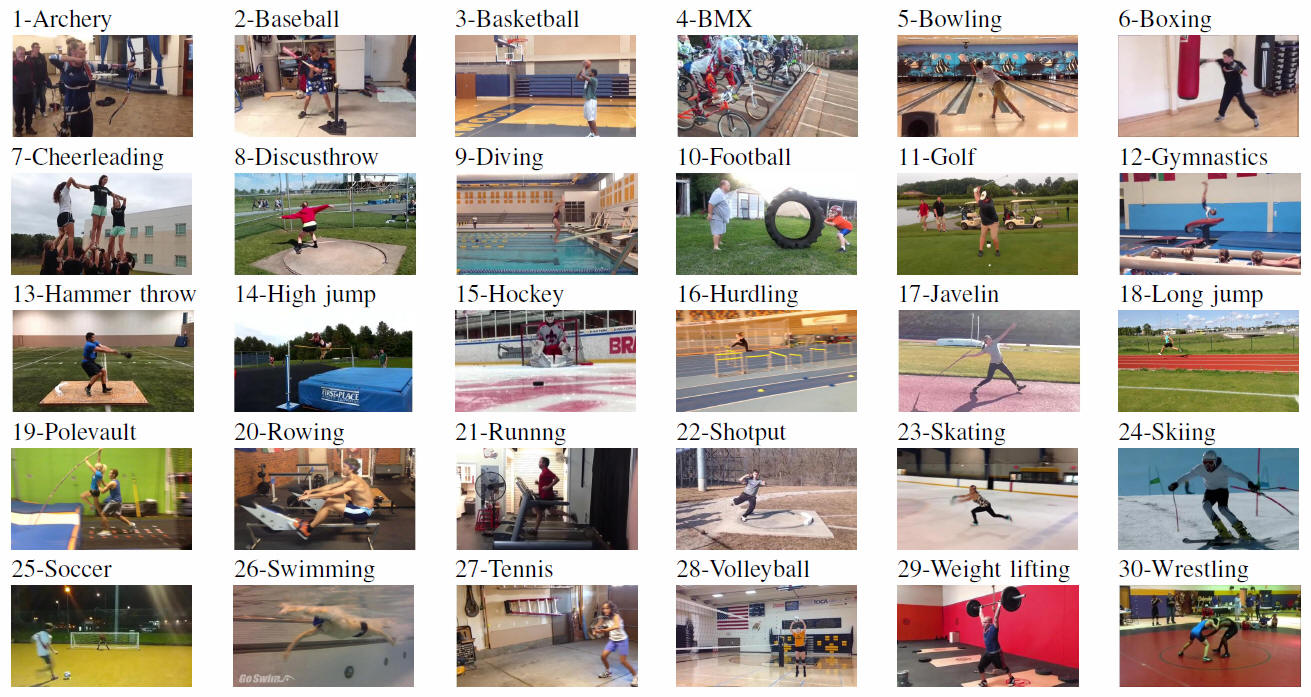
\includegraphics[height=8cm, width=0.99\linewidth]{svw-klatki.jpg}
    \caption{Klasy wraz z przykładowymi klatkami zbioru SVW}
    \label{fig:svw-klatki}
\end{figure}
\subsubsection{Statystyki zbioru}
Zbiór składa się łącznie z 4100 nagrań oraz 30 klas dyscyplin sportowych. Łączna długość nagrań wynosi 17.8 godzin. Rozmiary
poszczególnych klas zostały przedstawione na rysunku \ref{fig:raw-class-histogram}.
Twórcy zbioru danych dostarczyli również wyniki przeprowadzonych na zbiorze eksperymentów dla problemu rozpoznawania
dyscypliny sportu, jako metrykę bazową wynoszącą 61.53\%. Wynik ten został otrzymany przy pomocy kombinacji histogramów
zorientowanych gradientów (HOG), deskryptorów ruchu oraz deskryptorów trajektorii.
\begin{figure}[!h]
    \centering 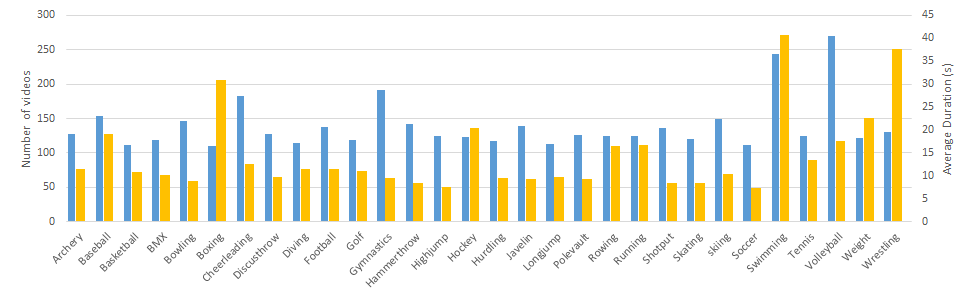
\includegraphics[width=0.90\linewidth]{stat1.png}
    \caption{Graf przedstawiający architekturę systemu}
    \label{fig:raw-class-histogram}
\end{figure}
\subsection{Ewaluacja modeli}
Zbiór danych SVW jest dostarczony razem z zalecanym podziałem przeznaczonym do walidacji krzyżowej o współczynniku
podziału wynoszącym $k = 3$. Metryki przedstawiające skuteczność modelu zostały wyznaczone przy pomocy podziału
zaproponowanego przez twórców zbioru składającego się z 70\% nagrań w zbiorze treningowym oraz 30\% nagrań w zbiorze testowym. 



